\part{Evolution and Stability}
\chapter{Evolution: Constraint Propagation and Characteristic Fronts}\markboth{\MakeUppercase{Chapter 19.\ Evolution}}{}
\label{ch:evolution}

\begin{usesbox}
\textbf{This chapter uses:} the spherical Einstein tensor in diagonal and double-null form (\cref{thm:einD,thm:einN}); the Yang--Mills field strength $F=\dd A+A\wedge A$ and the magnetic ansatz \eqref{eq:magansatz}; the Tolman universe and the throat (\cref{thm:tolman,thm:br}); the Gudermannian (\cref{thm:gudermann}); the null junction conditions (\cref{thm:null,thm:nullfront}).\\
\textbf{It provides:} the spherically symmetric EYM equations as a characteristic (Goursat) initial value problem; the proof that the constraints propagate, in both the double-null and the ADM form; the Tolman universe and the throat as solutions of the evolution equations in coordinates adapted to the junction; the characteristic fronts in the throat, which are lines of constant Mercator angle, $t=\ell\gd(z/\ell)$; and the transport of the jumps along the fronts.
\end{usesbox}

Chapters 13 to 18 treated a single moment of time. We now let the glued data evolve. The plan is the standard one for hyperbolic systems with constraints. First show that the evolution equations alone determine the solution and that the constraints, once satisfied, stay satisfied. Then identify the regions of the spacetime that are exactly known: those points whose past lies entirely in the Tolman part or entirely in the throat. The boundaries of these regions are null fronts from the junction sphere, and on the throat side these fronts are described by the Gudermannian of \cref{ch:hemisphere}.

\section{The Yang--Mills equation in double-null gauge}

Use the double-null metric \eqref{eq:nullmetric}, $\dd s^2=-2\Omega\,\dd u\,\dd v+r^2\dd\Omega^2$, and the magnetic ansatz with $w=w(u,v)$. Computing $F=\dd A+A\wedge A$ with the structure constants $\epsilon_{abc}$ of $\su(2)$, and then $D_\mu F^{\mu\nu}$, all components vanish identically except two, which are proportional to each other.

\begin{theorem}[Double-null Yang--Mills equation]\label{thm:ymnull}\ver\
For the magnetic ansatz in the double-null metric, the sixteen components $(D_\mu F^{\mu\nu})^a$ with $a=1,2,3$ and $\nu$ ranging over the coordinates reduce to the single equation
\[
w_{uv}=\frac{\Omega\,w(1-w^2)}{2r^2}.
\]
In the conformal gauge $\Omega=e^{2\sigma}$ the right-hand side is $e^{2\sigma}w(1-w^2)/(2r^2)$.
\end{theorem}
\begin{proof}
We use the densitised form $\partial_\mu(\sqrt{-g}F^{a\mu\nu})+\sqrt{-g}\,\epsilon_{abc}A^b_\mu F^{c\mu\nu}$, as in the proof of \cref{thm:4dcheck}, with $\sqrt{-g}=\Omega r^2s$ ($s=\sin\theta$) and $g^{uv}=-1/\Omega$. The field strength is the list of \cref{thm:ymstress}(i) with $(t,x)$ replaced by $(u,v)$.

\emph{The component $(a,\nu)=(1,\theta)$.} Raising indices, $\sqrt{-g}F^{1u\theta}=-s\,w_v$ and $\sqrt{-g}F^{1v\theta}=-s\,w_u$. Their divergence is $-2s\,w_{uv}$. The only colour term is $\epsilon_{123}A^2_\phi\sqrt{-g}F^{3\phi\theta}$. With $A^2_\phi=ws$ and $F^{3\phi\theta}=(1-w^2)/(r^4s)$, it equals $\Omega sw(1-w^2)/r^2$. Setting the sum to zero gives
\[
-2s\,w_{uv}+\frac{\Omega sw(1-w^2)}{r^2}=0 .
\]

\emph{The other components.} The component $(2,\phi)$ is the same equation without the factor $s$. The remaining components vanish identically for the reasons listed in the proof of \cref{thm:4dcheck}: either a $\partial_\theta$ of $\sin\theta$ cancels against the $\cos\theta$ in $A^3$, or every term contains a vanishing field component.
\end{proof}


There is no $w_u$ or $w_v$ on the right-hand side. This will be important: the $uv$-derivative of $w$ is determined by quantities that are continuous across a null front.

\section{A Goursat problem}

The remaining Einstein equations split into evolution equations, which are second order in $\partial_u\partial_v$, and two constraints along the null directions.

\begin{theorem}[Characteristic form of spherical EYM]\label{thm:goursat}\ver\
Let $C_u=r_{uu}-(\Omega_u/\Omega)r_u+2\ell^2w_u^2/r$ and $C_v$ the same with $u\leftrightarrow v$.
\begin{enumerate}[label=(\roman*)]
\item The $uu$ and $vv$ components of $G_{\mu\nu}-8\pi GT_{\mu\nu}$ are $-(2/r)C_u$ and $-(2/r)C_v$.
\item The $uv$ component of the Einstein equations is equivalent to
\[
r_{uv}=\frac{\Omega}{2r}\Bigl(\frac{\ell^2(1-w^2)^2}{r^2}-1\Bigr)-\frac{r_ur_v}{r},
\]
and the $\theta\theta$ component, given this, to
\[
\Omega_{uv}=\frac{\Omega_u\Omega_v}{\Omega}-\frac{2\Omega\,r_{uv}}{r}-\frac{\Omega^2\ell^2(1-w^2)^2}{r^4}.
\]
\item Together with \cref{thm:ymnull}, these three equations express $r_{uv}$, $\Omega_{uv}$, $w_{uv}$ through the fields and their first derivatives.
\end{enumerate}
\end{theorem}
\begin{proof}
\emph{(i)} By the proof of \cref{thm:null}(ii), $G_{uu}=-\frac2r(r_{uu}-\frac{\Omega_u}\Omega r_u)$. By \cref{thm:ymstress}(iii), $8\pi GT_{uu}=2\ell^2\hat T_{uu}=4\ell^2w_u^2/r^2$. Subtracting,
\[
G_{uu}-8\pi GT_{uu}=-\frac2r\Bigl(r_{uu}-\frac{\Omega_u}\Omega r_u+\frac{2\ell^2w_u^2}r\Bigr)=-\frac2rC_u .
\]

\emph{(ii)} The $uv$ equation is the mixed equation of \cref{thm:null}(iii), solved for $r_{uv}$. For the $\theta\theta$ equation we need the curvature of $h=-2\Omega\,\dd u\,\dd v$, which is conformal to the flat metric with conformal factor $\Omega$:
\[
{}^{(2)}\!R=\frac2\Omega(\log\Omega)_{uv}=\frac{2\Omega_{uv}}{\Omega^2}-\frac{2\Omega_u\Omega_v}{\Omega^3}.
\]
Then
\[
G^\theta{}_\theta=\frac{\Box r}r-\frac12{}^{(2)}\!R=-\frac{2r_{uv}}{\Omega r}-\frac{\Omega_{uv}}{\Omega^2}+\frac{\Omega_u\Omega_v}{\Omega^3}.
\]
Set this equal to $8\pi GT^\theta{}_\theta=\ell^2(1-w^2)^2/r^4$ and multiply by $\Omega^2$.

\emph{(iii)} The three equations are solved for $r_{uv}$, $\Omega_{uv}$ and $w_{uv}$. Their right sides contain only the fields and their first derivatives.
\end{proof}


Equations of the form $f_{uv}=F(f,f_u,f_v)$ define a Goursat problem: one prescribes $f$ on two intersecting null lines $u=u_0$ and $v=v_0$, and the solution exists and is unique in a neighbourhood of the corner \cite{Goursat}. The constraints restrict the data on the two lines.

\begin{theorem}[The constraints propagate]\label{thm:constrprop}\ver\
\begin{enumerate}[label=(\roman*)]
\item If $r_{uv}$, $\Omega_{uv}$ and $w_{uv}$ satisfy the three evolution equations of \cref{thm:goursat}, then
\[
\partial_vC_u=-\frac{r_v}{r}\,C_u,\qquad \partial_uC_v=-\frac{r_u}{r}\,C_v .
\]
The same conclusion holds starting directly from the $uv$ and $\theta\theta$ Einstein equations and the Yang--Mills equation for $F=\dd A+A\wedge A$.
\item Consequently, if $C_u=0$ on the initial line $v=v_0$ and $r>0$, then $C_u=0$ everywhere along each line of constant $u$: $C_u$ satisfies a linear homogeneous ODE with zero initial value.
\item In the ADM formulation with zero shift and unit lapse, metric $-\dd t^2+A^2\dd x^2+R^2\dd\Omega^2$, extrinsic curvature components $K^x{}_x$, $K^\theta{}_\theta$, and Yang--Mills momentum $P=A\,\partial_tw$, the Hamiltonian constraint $\mathcal H$ and the momentum constraint $\mathcal M$ satisfy
\[
\partial_t\mathcal H=2K\mathcal H-4\frac{DR}{R}\mathcal M-2D\mathcal M,\qquad \partial_t\mathcal M=2(K^x{}_x+K^\theta{}_\theta)\mathcal M-\tfrac12D\mathcal H,
\]
with $D=A^{-1}\partial_x$ and $K=K^x{}_x+2K^\theta{}_\theta$.
\end{enumerate}
\end{theorem}
\begin{proof}
\emph{(i)} Write $P=(1-w^2)^2$ and $F=\frac\Omega{2r}\bigl(\frac{\ell^2P}{r^2}-1\bigr)-\frac{r_ur_v}r$, so that $r_{uv}=F$. Differentiate
\[
C_u=r_{uu}-\frac{\Omega_u}\Omega r_u+\frac{2\ell^2w_u^2}r
\]
in $v$. Replace $r_{uuv}$ by $\partial_uF$, $(\Omega_u/\Omega)_v=\Omega_{uv}/\Omega-\Omega_u\Omega_v/\Omega^2$ by $-2r_{uv}/r-\Omega\ell^2P/r^4$ (the $\theta\theta$ equation), and $w_{uv}$ by \cref{thm:ymnull}. Then four groups of terms cancel.
\begin{itemize}[nosep]
\item The Yang--Mills terms: $\partial_u$ of $P$ inside $F$ gives $-2\Omega\ell^2ww_u(1-w^2)/r^3$. The term $4\ell^2w_uw_{uv}/r$ gives the opposite.
\item The terms $\pm\Omega\ell^2Pr_u/r^4$.
\item From $-r_ur_{uv}/r+2r_ur_{uv}/r=r_uF/r$: this cancels the terms of $\partial_uF$ that contain $\Omega r_u/(2r^2)$ and $r_u^2r_v/r^2$.
\item From $-\frac{\Omega_u}\Omega r_{uv}=-\frac{\Omega_u}\Omega F$: its first part cancels the $\Omega_u$ term of $\partial_uF$.
\end{itemize}
What survives is
\[
-\frac{r_vr_{uu}}r+\frac{\Omega_u}\Omega\frac{r_ur_v}r-\frac{2\ell^2w_u^2r_v}{r^2}=-\frac{r_v}rC_u .
\]
The equation for $C_v$ follows by symmetry.

\emph{(ii)} By (i), $\partial_v(rC_u)=r_vC_u+r\,\partial_vC_u=0$. So $rC_u$ is constant along each line of constant $u$, and it vanishes because it vanishes on $v=v_0$. Since $r>0$, $C_u=0$.

\emph{(iii)} Outline. The contracted Bianchi identity, together with $\nabla_\mu T^{\mu\nu}=0$ (which holds by the Yang--Mills equation), gives $\nabla_\mu(G^{\mu\nu}-8\pi GT^{\mu\nu})=0$. When the evolution equations hold, only the components $\mathcal H$ and $\mathcal M$ of $G-8\pi GT$ can be nonzero. The $t$ and $x$ components of the identity then become a linear system for them. Its coefficients are Christoffel symbols of the metric, which are $K^x{}_x$, $K^\theta{}_\theta$ and $DR/R$. Writing it out gives the two stated equations; Lean checks them by expansion. The conclusion that zero constraints stay zero is the standard uniqueness for such linear symmetric hyperbolic systems \ext.
\end{proof}


\Cref{thm:constrprop} is the spherical form of the contracted Bianchi identity $\nabla_\mu G^{\mu\nu}=0$, which we proved in general in \cref{ch:fields}. Here it appears as an explicit, checkable statement for the reduced equations. The existence and uniqueness of solutions to the full non-linear system are external input \ext; the classical reference is Choquet-Bruhat's theorem \cite{ChoquetBruhat1952}, and for data with a jump in second derivatives one needs the low-regularity theory, which in spherical symmetry is due to Christodoulou \cite{Christodoulou1993}.

\section{The two exact solutions as evolutions}

In the diagonal gauge $-N^2\dd t^2+A^2\dd x^2+R^2\dd\Omega^2$ both pieces of the glued slice evolve explicitly.

\begin{theorem}[Tolman side]\label{thm:tolmanevo}\ver\
Take conformal time $\eta$ and polar angle $\chi$, $N=A=a(\eta)$, $R=a(\eta)\sin\chi$, $w=\cos\chi$.
\begin{enumerate}[label=(\roman*)]
\item The $tt$ component of the field equations is equivalent to the Friedmann equation $a'^2+a^2=\ell^2$; the $\chi\chi$ and $\theta\theta$ components are both equivalent to $2aa''-a'^2+a^2+\ell^2=0$; the $t\chi$ component holds identically.
\item Together these give $a''=-a$, and the time-symmetric solution with $a(0)=\ell$ is $a=\ell\cos\eta$.
\item The proper time at the centre is $\tau=\ell\sin\eta$, so the universe recollapses at $\eta=\pi/2$ after proper time $\ell$. The Yang--Mills energy density is $\rho=3/(2g^2a^4)$, which diverges as $\eta\to\pi/2$.
\item $\ell<\pi\ell/2$: the crunch occurs before the time $\pi\ell/2$ at which the throat's synchronous coordinates (below) break down.
\end{enumerate}
\end{theorem}
\begin{proof}
For the metric $a^2(-\dd\eta^2+\dd\chi^2+\sin^2\chi\,\dd\Omega^2)$ the standard closed FRW expressions in conformal time are
\[
G_{\eta\eta}=\frac{3(a'^2+a^2)}{a^2},\qquad G^\chi{}_\chi=G^\theta{}_\theta=-\frac1{a^2}\Bigl(\frac{2a''}a-\frac{a'^2}{a^2}+1\Bigr),\qquad G_{\eta\chi}=0 .
\]
By \cref{thm:tolmanstress}, $8\pi G\rho=8\pi G\cdot\frac3{2g^2a^4}=\frac{3\ell^2}{a^4}$, and $p=\rho/3$ in every direction. Also $T_{\eta\chi}=0$, since $w$ does not depend on $\eta$.

\emph{(i)} The $\eta\eta$ equation is $3(a'^2+a^2)/a^2=8\pi G\rho\,a^2=3\ell^2/a^2$. The spatial equations are $-(2a''/a-a'^2/a^2+1)/a^2=\ell^2/a^4$, that is, $2aa''-a'^2+a^2+\ell^2=0$.

\emph{(ii)} Insert $a'^2=\ell^2-a^2$ into the spatial equation: $2aa''+2a^2=0$. The solution with $a(0)=\ell$ and $a'(0)=0$ is $\ell\cos\eta$.

\emph{(iii)} $\dd\tau=a\,\dd\eta=\ell\cos\eta\,\dd\eta$, so $\tau=\ell\sin\eta$, which is $\ell$ at $\eta=\pi/2$. The density $3/(2g^2\ell^4\cos^4\eta)$ tends to infinity there.

\emph{(iv)} $\ell<\frac\pi2\ell$, since $\pi>2$.
\end{proof}


\begin{theorem}[Throat side]\label{thm:throatevo}\ver\
Take $N=1$, $A=\cos(t/\ell)$, $R=\ell$, $w=0$, i.e.\ the metric
\[
\dd s^2=-\dd t^2+\cos^2(t/\ell)\,\dd z^2+\ell^2\dd\Omega^2 .
\]
All components of the EYM equations hold. This is $\mathrm{AdS}_2\times S^2$ in Gaussian normal coordinates adapted to the time-symmetric slice $t=0$; the coordinates are valid for $|t|<\pi\ell/2$.
\end{theorem}
\begin{proof}
The two-dimensional part $-\dd t^2+A^2\dd z^2$ with $A=\cos(t/\ell)$ has ${}^{(2)}\!R=2\ddot A/A=-2/\ell^2$, so it is $\mathrm{AdS}_2$ of radius $\ell$. Since $R=\ell$ is constant, every derivative of $R$ vanishes in the $2+2$ formulas of \cref{thm:einD}. They give
\[
G^a{}_b=-\frac{\delta^a{}_b}{\ell^2},\qquad G^\theta{}_\theta=-\frac12{}^{(2)}\!R=\frac1{\ell^2}.
\]
With $w=0$ the stress is $\rho\operatorname{diag}(-1,-1,1,1)$ with $8\pi G\rho=1/\ell^2$ (\cref{thm:br}). So all components agree. The Yang--Mills equation holds trivially for $w=0$.

The lapse is $1$, so $t$ is proper time along the normals, and $\dot A(0)=0$, so the slice $t=0$ is time symmetric. The metric degenerates where $\cos(t/\ell)=0$.
\end{proof}


\section{Characteristic fronts in the throat}

At $t=0$ the two pieces are joined at the junction sphere. The null fronts leaving it bound the regions where the solution is known exactly. On the throat side, a right-moving null curve satisfies $\dd z/\dd t=1/\cos(t/\ell)$.

\begin{theorem}[Fronts as Mercator lines]\label{thm:fronts}\ver\
\begin{enumerate}[label=(\roman*)]
\item The null curve through $z=0$ at $t=0$ is $z=\ell\,\operatorname{arsinh}\tan(t/\ell)$, equivalently
\[
t=\ell\,\gd(z/\ell),
\]
and this is the only future-directed right-moving null curve through the origin within the strip $|t|<\pi\ell/2$. The two descriptions are mutually inverse on that strip.
\item The identities $\tan\gd y=\sinh y$, $\cos\gd y=\operatorname{sech}y$, $\gd'y=\cos\gd y$ and $\sqrt{1+\tan^2u}=1/\cos u$ (for $\cos u>0$) are the ones behind (i).
\item (Mercator) With $t=\ell\gd(y/\ell)$, $\dd t/\dd y=\cos(t/\ell)$, so
\[
-\dd t^2+\cos^2(t/\ell)\,\dd z^2=\cos^2(t/\ell)\bigl(-\dd y^2+\dd z^2\bigr).
\]
The same Gudermann map that makes the sphere $\dd\varphi^2+\cos^2\varphi\,\dd\lambda^2$ conformally flat in Mercator's coordinates makes the two-dimensional part of the throat conformally flat.
\item Fronts entering a throat segment of length $L$ from both ends meet at $t_*=\ell\gd(L/(2\ell))$, and only then. For every $z$, the arrival time $\ell\gd(z/\ell)$ is less than $\pi\ell/2$.
\item On the Tolman side the inward front from the junction is $\chi=\pi/2-\eta$; it reaches the centre exactly at the crunch $\eta=\pi/2$.
\item As $\ell\to\infty$: $\ell\gd(z/\ell)\to z$, $\ell\operatorname{arsinh}\tan(t/\ell)\to t$, $\cos^2(t/\ell)\to1$ and $\operatorname{sech}(z/\ell)\to1$, the flat light cone.
\end{enumerate}
\end{theorem}
\begin{proof}
\emph{(i)} We must solve $\dd z/\dd t=\sec(t/\ell)$ with $z(0)=0$. For $\cos x>0$,
\[
\frac{\dd}{\dd x}\operatorname{arsinh}(\tan x)=\frac{\sec^2x}{\sqrt{1+\tan^2x}}=\sec x .
\]
So $z=\ell\operatorname{arsinh}\tan(t/\ell)$, and by uniqueness for this ODE it is the only solution. Solving for $t$ gives $\tan(t/\ell)=\sinh(z/\ell)$, that is, $t=\ell\arctan\sinh(z/\ell)=\ell\gd(z/\ell)$.

\emph{(ii)} By definition $\gd y=\arctan\sinh y$, so $\tan\gd y=\sinh y$. Then $\cos\gd y=1/\sqrt{1+\sinh^2y}=\operatorname{sech}y$. Finally $\gd'y=\cosh y/(1+\sinh^2y)=\operatorname{sech}y$.

\emph{(iii)} By (ii), $\dd t/\dd y=\gd'(y/\ell)=\cos\gd(y/\ell)=\cos(t/\ell)$. So $\dd t^2=\cos^2(t/\ell)\,\dd y^2$.

\emph{(iv)} The fronts from $z=0$ and $z=L$ are mirror images in $z=L/2$, so they meet there, at time $\ell\gd(L/(2\ell))$. Since $\gd<\pi/2$, every arrival time is less than $\pi\ell/2$.

\emph{(v)} In conformal coordinates the null curves are $\chi\pm\eta=$ const. The inward one through $(\eta,\chi)=(0,\pi/2)$ is $\chi=\pi/2-\eta$, which reaches $\chi=0$ at $\eta=\pi/2$.

\emph{(vi)} Each function is $x+O(x^3)$, or $1+O(x^2)$ for the last two, with $x=z/\ell$ or $t/\ell$. Multiplying by $\ell$ and letting $\ell\to\infty$ gives the limits.
\end{proof}


\begin{figure}[t]
\centering
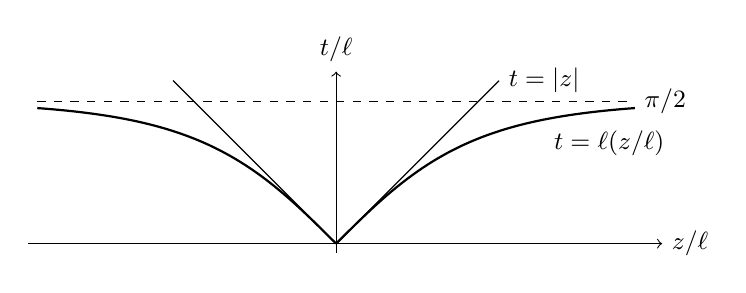
\begin{tikzpicture}[scale=1.15]
\draw[->] (-3.4,0) -- (3.6,0) node[right] {\small $z/\ell$};
\draw[->] (0,-0.1) -- (0,1.9) node[above] {\small $t/\ell$};
\draw[dashed] (-3.3,1.5708) -- (3.3,1.5708) node[right] {\small $\pi/2$};
\draw[thick,domain=0:3.3,samples=60] plot (\x,{2*atan(tanh(\x/2))*3.14159/180});
\draw[thick,domain=-3.3:0,samples=60] plot (\x,{-2*atan(tanh(\x/2))*3.14159/180});
\draw[thin,domain=0:1.8,samples=30] plot (\x,\x);
\draw[thin,domain=-1.8:0,samples=30] plot (\x,-\x);
\node[right] at (1.8,1.8) {\small $t=|z|$};
\node[below right] at (2.3,1.35) {\small $t=\ell\gd(z/\ell)$};
\end{tikzpicture}
\caption{Null fronts from $z=0$ in the throat (thick), compared with the flat light cone (thin). In the synchronous coordinates the front approaches $t=\pi\ell/2$ but never reaches it.}
\label{fig:fronts}
\end{figure}

\Cref{thm:fronts} is where the geometry of \cref{ch:hemisphere} returns. There the Gudermannian related the rapidity $\zeta$ of a particle to the polar angle $\chi$ on the hemisphere. Here the same function relates the proper distance $z/\ell$ along the throat to the arrival time $t/\ell$ of a light signal. The throat's time plays the role of the circular angle and its space the role of rapidity, which is the statement that $\mathrm{AdS}_2$ is Lorentzian hyperbolic space with a circle of time.

\section{Jumps along the fronts}

\begin{proposition}[Transport of jumps]\label{prop:jumps}\ver\
\begin{enumerate}[label=(\roman*)]
\item If on both sides of a front $u=u_0$ the derivatives $\partial_v w_u^\pm$ equal $e^{2\sigma}w(1-w^2)/(2r^2)$, with $r,\sigma,w$ continuous, then the jump $[w_u]$ is independent of $v$. (A version in the evaluation-map formulation of \cref{ch:junctions} is also listed; see the remark there on its hypotheses.)
\item If the constraint $r_{uu}=2\sigma_ur_u-2\ell^2w_u^2/r$ holds on both sides with $r,\sigma_u,r_u$ continuous, then $[r_{uu}]=-(2\ell^2/r)[w_u^2]$.
\end{enumerate}
\end{proposition}
\begin{proof}
\emph{(i)} $\partial_v(w_u^+-w_u^-)=0$, because both sides equal the same continuous function. So the jump is constant in $v$.

\emph{(ii)} Subtract the two constraints. The term $2\sigma_ur_u$ is continuous and drops out, leaving $[r_{uu}]=-\frac{2\ell^2}r[w_u^2]$.
\end{proof}


With the corner values from \cref{thm:nullfront} this gives $[w_u]=1/(\sqrt2\ell)$ and $[r_{uu}]=-1/\ell$ along the whole front. The glued spacetime is therefore smooth except across two null hypersurfaces, on which second derivatives jump by fixed amounts. This is a weak discontinuity in the sense of hyperbolic PDE \cite{CourantHilbert2}, the gravitational analogue of a sound front.

\begin{litbox}
The characteristic initial value problem for Einstein's equations goes back to Sachs and Bondi; in spherical symmetry, the double-null formulation of the Einstein--scalar field system is due to Christodoulou \cite{Christodoulou1993}, and it has been applied to EYM in numerical studies of critical collapse \cite{ChoptuikChmajBizon1996}. Constraint propagation for the ADM equations is classical \cite{Frittelli1997}. Mercator's projection and the Gudermannian are of course old. What we believe is new is: the reduction of spherical EYM in double-null gauge to a Goursat system, with the propagation of the null constraints, checked for the full field strength $F=\dd A+A\wedge A$ (\cref{thm:ymnull,thm:goursat,thm:constrprop}); the evolution of the glued slice with explicit exact regions; and the observation that the light fronts of the throat are Mercator lines, $t=\ell\gd(z/\ell)$, the same function that links rapidity and hemisphere angle in \cref{ch:hemisphere} (\cref{thm:fronts}).
\end{litbox}

\section*{What this chapter passes on}
\begin{itemize}[nosep]
\item $w_{uv}=\Omega w(1-w^2)/(2r^2)$ and the Goursat form of the field equations (\cref{thm:ymnull,thm:goursat}).
\item The constraints propagate (\cref{thm:constrprop}).
\item Tolman side: $a=\ell\cos\eta$, crunch at proper time $\ell$; throat side: $-\dd t^2+\cos^2(t/\ell)\dd z^2+\ell^2\dd\Omega^2$ (\cref{thm:tolmanevo,thm:throatevo}).
\item Fronts $t=\ell\gd(z/\ell)$, meeting at $\ell\gd(L/2\ell)<\pi\ell/2$ (\cref{thm:fronts}).
\item Fixed jumps $[w_u]$, $[r_{uu}]$ along the fronts (\cref{prop:jumps}).
\end{itemize}

\section*{Exercises}
\begin{exercise}
Show that $z(t)=\ell\operatorname{arsinh}\tan(t/\ell)$ satisfies $\dd z/\dd t=1/\cos(t/\ell)$ for $|t|<\pi\ell/2$.
\end{exercise}
\begin{exercise}
From $a'^2+a^2=\ell^2$ and $2aa''-a'^2+a^2+\ell^2=0$ derive $a''=-a$.
\end{exercise}
\begin{exercise}
Prove $\ell\gd(z/\ell)<\pi\ell/2$ for all real $z$ and $\ell>0$.
\end{exercise}
\begin{exercise}
Show that the front $\chi=\pi/2-\eta$ is null for the metric $a^2(-\dd\eta^2+\dd\chi^2)$, and that a continuous $\chi'$ with $\chi'^2=1$ and $\chi'(0)=-1$ is identically $-1$.
\end{exercise}

\begin{checklist}
\chk{AlphaS5_Evolution:eps3_table}{The structure constants $\epsilon_{abc}$ of $\su(2)$ as a table.}
\chk{AlphaS5_Evolution:ymN_*}{The sixteen components of the double-null Yang--Mills equation: fourteen vanish, two reduce to $w_{uv}=\Omega w(1-w^2)/(2r^2)$ (sixteen statements).$^*$}
\chk{AlphaS5_Evolution:goursat_W}{Goursat form of the Yang--Mills equation.$^*$}
\chk{AlphaS5_Evolution:fw_eq}{The same right-hand side in conformal gauge $\Omega=e^{2\sigma}$.}
\chk{AlphaS5_Evolution:constraint_uu,AlphaS5_Evolution:constraint_vv}{The $uu$, $vv$ Einstein equations are $-(2/r)C_u$, $-(2/r)C_v$ (two statements).$^*$}
\chk{AlphaS5_Evolution:goursat_r}{Goursat form for $r_{uv}$.$^*$}
\chk{AlphaS5_Evolution:goursat_Om}{Goursat form for $\Omega_{uv}$.$^*$}
\chk{AlphaS5_Evolution:constraint_prop_u,AlphaS5_Evolution:constraint_prop_v}{$\partial_vC_u=-(r_v/r)C_u$ and $\partial_uC_v=-(r_u/r)C_v$ (two statements).$^*$}
\chk{AlphaS5_Curvature:constraint_prop_from_eqs}{The same, directly from the field equations with $F=\dd A+A\wedge A$.$^*$}
\chk{AlphaS5_Evolution:constraint_transport}{Vanishing initial constraint stays zero.$^*$}
\chk{AlphaIV_Propagation:deriv_inv,AlphaIV_Propagation:deriv_ofNat}{Derivation of an inverse and of an integer (two lemmas).}
\chk{AlphaIV_Propagation:hamiltonian_propagation}{$\partial_t\mathcal H$ in terms of $\mathcal H,\mathcal M$.$^*$}
\chk{AlphaIV_Propagation:momentum_propagation}{$\partial_t\mathcal M$ in terms of $\mathcal H,\mathcal M$.$^*$}
\chk{AlphaS5_Evolution:capSph}{The Tolman data define a spherically symmetric diagonal metric.}
\chk{AlphaS5_Evolution:cap_00}{$tt$ component $\Leftrightarrow$ $a'^2+a^2=\ell^2$.$^*$}
\chk{AlphaS5_Evolution:cap_11,AlphaS5_Evolution:cap_22}{$\chi\chi$, $\theta\theta$ components $\Leftrightarrow$ $2aa''-a'^2+a^2+\ell^2=0$ (two statements).$^*$}
\chk{AlphaS5_Evolution:cap_01}{The $t\chi$ component holds identically.}
\chk{AlphaS5_Evolution:cap_accel}{$a''=-a$.}
\chk{AlphaS5_Evolution:cap_unique}{Time-symmetric solution $a=\ell\cos\eta$ is unique.$^*$}
\chk{AlphaS5_Evolution:cap_proper_time,AlphaIV:cap_lifetime}{Proper time $\ell\sin\eta$; crunch at $\eta=\pi/2$ after proper time $\ell$ (two statements).}
\chk{AlphaS5_Evolution:cap_density}{Energy density $3/(2a^4)$.$^*$}
\chk{AlphaS5_Evolution:cap_crunch}{The density diverges at the crunch.$^*$}
\chk{AlphaS5_Evolution:t_sing_lt}{$\ell<\pi\ell/2$.}
\chk{AlphaS5_Evolution:neckSph}{The throat data define a spherically symmetric diagonal metric.}
\chk{AlphaS5_Evolution:neck_00,AlphaS5_Evolution:neck_11,AlphaS5_Evolution:neck_22,AlphaS5_Evolution:neck_01}{The throat in synchronous coordinates satisfies all components (four statements).$^*$}
\chk{AlphaIV:front_deriv}{$\dd z/\dd t=1/\cos(t/\ell)$ along $z=\ell\operatorname{arsinh}\tan(t/\ell)$.$^*$}
\chk{AlphaIV:tan_gd,AlphaIV:gd_deriv,AlphaIV:gd_deriv_zero,AlphaIV:gd_zero,AlphaIV:sqrt_one_add_tan_sq}{Identities for $\gd$ and $\tan$ (five statements).}
\chk{AlphaS5_Evolution:cos_gd,AlphaS5_Evolution:front_deriv_zero}{$\cos\gd y=\operatorname{sech}y$; derivative of $\operatorname{arsinh}\circ\tan$ at $0$ (two statements).}
\chk{AlphaS5_Evolution:front_gd_inv,AlphaS5_Evolution:gd_front_inv}{The front and $\ell\gd(\cdot/\ell)$ are mutually inverse (two statements).$^*$}
\chk{AlphaS5_Evolution:mercator,AlphaS5_Evolution:neck_mercator}{Mercator: $\gd'=\cos\circ\gd$, and the throat metric becomes conformally flat (two statements).$^*$}
\chk{AlphaS5_Evolution:null_curve_unique}{Uniqueness of the front $t=\ell\gd(z/\ell)$.$^*$}
\chk{AlphaS5_Evolution:fronts_meet_iff}{Fronts meet iff $t=\ell\gd(L/2\ell)$.$^*$}
\chk{AlphaIV:fronts_meet_before,AlphaIV:arrival_bound}{Meeting and arrival times are below $\pi\ell/2$ (two statements).$^*$}
\chk{AlphaS5_Evolution:center_before_front}{Before the crunch the centre is outside the front.}
\chk{AlphaS5_Evolution:flat_clock,AlphaS5_Evolution:flat_front,AlphaS5_Evolution:flat_metric}{Flat limits $\ell\to\infty$ (three statements).}
\chk{AlphaIV:jump_const}{$[w_u]$ is constant along a front.$^*$}
\chk{AlphaS5_Final:wave_jump_final}{The same in the evaluation-map formulation (hypotheses not satisfiable by non-constant fields; see \cref{ch:junctions}).}
\chk{AlphaIV:ruu_jump}{$[r_{uu}]=-(2/r)[w_u^2]$ (in units with $\ell$ absorbed).}
\end{checklist}
